% \iffalse meta-comment
%
% Copyright (C) 2021 MeteoSwiss, originally written by Frédéric P.A. Vogt
%
% This file may be distributed and/or modified under the
% conditions of the BSD-3-Clause License.
% The terms of this license are available at:
%
% https://opensource.org/licenses/BSD-3-Clause
%
% SPDX-License-Identifier: BSD-3-Clause
%
%
% \fi
%
% \iffalse
%<package>\NeedsTeXFormat{LaTeX2e}[2005/12/01]
%<package>\ProvidesPackage{metsymb}
%<package>     [2021/08/24 v1.0 The meteorological symbols package]
%
%<*driver>
\documentclass{ltxdoc}
\usepackage[margin=1.in]{geometry} % For more reasonable margins
\usepackage{tocloft} % For a better table of content in the doc
\renewcommand{\cftsecleader}{\cftdotfill{\cftdotsep}} % Idem
\usepackage{color} % For using colors
\usepackage{tabularx} % For the tables
\usepackage{graphicx} % For the demo Python plot
\usepackage{listings}% For including code
\lstset{ 
  basicstyle=\footnotesize,        % the size of the fonts that are used for the code
  frame=single,                          % add a frame around code
  }
\usepackage{hyperref} % For the colored table of contents
\hypersetup{
    colorlinks=true,
    linkcolor=red,
    %filecolor=magenta,      
    urlcolor=blue,
    %pdftitle={Overleaf Example},
    %pdfpagemode=FullScreen,
    }
\usepackage{metsymb}
\EnableCrossrefs
\CodelineIndex
\RecordChanges
\begin{document}
\DocInput{metsymb.dtx}
\end{document}
%</driver>
% \fi
%
% \CheckSum{30}
%
% \CharacterTable
% {Upper-case \A\B\C\D\E\F\G\H\I\J\K\L\M\N\O\P\Q\R\S\T\U\V\W\X\Y\Z
% Lower-case \a\b\c\d\e\f\g\h\i\j\k\l\m\n\o\p\q\r\s\t\u\v\w\x\y\z
% Digits \0\1\2\3\4\5\6\7\8\9
% Exclamation \! Double quote \" Hash (number) \#
% Dollar \$ Percent \% Ampersand \&
% Acute accent \' Left paren \( Right paren \)
% Asterisk \* Plus \+ Comma \,
% Minus \- Point \. Solidus \/
% Colon \: Semicolon \; Less than \<
% Equals \= Greater than \> Question mark \?
% Commercial at \@ Left bracket \[ Backslash \\
% Right bracket \] Circumflex \^ Underscore \_
% Grave accent \` Left brace \{ Vertical bar \|
% Right brace \} Tilde \~}
%
%
% \changes{v1.0}{2021/08/24}{Initial version, with okta symbols.}
%
% \GetFileInfo{metsymb.sty}
%
% \DoNotIndex{}
%
% \title{The \textsf{metsymb} package\thanks{This document
% corresponds to \textsf{metsymb}~\fileversion,
% dated \filedate.}}
% \author{Frédéric P.A. Vogt \\ \texttt{frederic.vogt@meteoswiss.ch}}
%
% \maketitle
%
% \begin{abstract}
% \noindent This package introduces commands to generate meteorological symbols. As of \today, these include: okta symbols (\zerookta, \oneokta, \twooktas, \ldots). This package effectively introduces a new font in which each symbol is assigned to a glyph, which can then be called individually from \LaTeX\ documents via dedicated new commands.
% \end{abstract}
%
% \tableofcontents
% 
% \section{Introduction}
%
% The creation of this package was initially motivated by the fact that, as of August 24, 2021, there were no dedicated Unicode element for all of \href{https://en.wikipedia.org/wiki/Okta}{the ten okta symbols}. To the best of my knowledge, no \LaTeX\ package provides a uniform set of these ten symbols either\footnote{If you know of one, please let me know and I shall list it here !}.\\ 
%
% \noindent This humble package is a direct attempt to remedy --in part-- to this sad state of affair. A new font, created using FontForge\footnote{\url{https://fontforge.org/en-US/}}, is used to generate the new symbols, and assign them to individual glyphs. Individual glyphs can then be called individually using dedicated \LaTeX\ commands.
%
% \section{Usage}
%
% Using the \textsf{metsymb} package is straightforward. By importing it via a not-so-surprising \texttt{\textbackslash usepackage\{metsymb\}} in the preamble of your documents, you will gain access to the commands listed in Table~\ref{tbl:comm}.
%
% \begin{table}[htb!]
% \centering
% \caption{\textsf{metsymb} commands for the okta symbols.}\label{tbl:comm}
% \vspace{5pt}
% \begin{tabular}{c l c l}
% \zerookta & |\zerookta| &  \fiveoktas & |\fiveoktas|\\
% \oneokta & |\oneokta| & \sixoktas & |\sixoktas|\\
% \twooktas & |\twooktas| & \sevenoktas & |\sevenoktas|\\
% \threeoktas & |\threeoktas| & \eightoktas & |\eightoktas|\\
% \fouroktas & |\fouroktas| & \nineoktas & |\nineoktas|
% 
% \end{tabular}
%\end{table}
%
% \subsection{Using \textsf{metsymb} with \textsf{matplotlib}}
% 
%
% $ $\\
% The assembly of a dedicated font to store the \textsf{metsymb} symbols\footnote{instead of a simpler \texttt{tikz} approach, \href{https://tex.stackexchange.com/questions/610992/creating-new-symbols-with-full-font-metrics-and-vector-quality}{for example}} is directly motivated by the fact that \textsf{matplotlib} \href{https://stackoverflow.com/questions/68769147/tikzpicture-cropped-from-dvi-when-used-in-matplotlib-plt-text}{requires proper font metrics} to include symbols in Python plots.\\
%
% \noindent Hence, \textsf{metsymb} can be used to include meteorological symbols inside Python plots, provided that the use of a system-wide \LaTeX\ installation is enabled prior to generating the plots. Modifying the \texttt{rcparams} elements is one way to do so, as illustrated in the following minimal working example (stored in \texttt{metsymb\_mwe.py}; see Fig.~\ref{fig:mwe} for the result):
%
% \lstinputlisting[language=Python]{metsymb_mwe.py}
%
% \noindent where \texttt{metsymb\_mwe.mplstyle} contains:
% 
% \lstinputlisting[language=Python]{metsymb_mwe.mplstyle}
%
% \begin{figure}[htb!]
% \centerline{
\includegraphics{metsymb_mwe.pdf}}
% \caption{Result of the \texttt{metsymb\_mwe.py} demonstration script, illustrating how the \textsf{metsymb} package can be used with \textsf{matplotlib}.}\label{fig:mwe}
% \end{figure}
% \begin{center}
%    \color{red}
%  \textbf{WARNING !}\\ The use of \texttt{text.latex.preamble} in the \texttt{rcparams} of \textsf{matplotlib} is not an officially supported feature of that package ! Proceed at your own risks ! \end{center}
%
% \section{Code development and bug reports}
% The \textsf{metsymb} package is being developed inside a dedicated Github repository under the MeteoSwiss organization, located at: \url{https://github.com/MeteoSwiss/metsymb}. User contributions are welcome and will be examined in details. So are bug reports and suggestions for new symbols, which are best submitted as \textit{Github Issues} directly on the code's repo at: \url{https://github.com/MeteoSwiss/metsymb/issues}
%
% \section{License and copyright}
% The copyright (2021) of \textsf{metsymb} is owned by MeteoSwiss. The code, originally written by Frédéric P.A. Vogt, is released under the terms of the BSD-3-Clause License, available at \url{https://opensource.org/licenses/BSD-3-Clause}. 
%
% \section{Ackowledgments}
% The following resources proved immensely useful to assemble the first version of this package:
% \begin{itemize}
% \item  \textit{How to Package Your \LaTeX Package}, Scott Pakin (2015): \url{https://mirror.foobar.to/CTAN/info/dtxtut/dtxtut.pdf}
% \item The FontForge documentation, and in particular the \textit{FontForge and TeX} article: \url{https://fontforge.org/docs/techref/PfaEdit-TeX.html}
%\item The \textit{\TeX\ font errors: Cheatsheet}: \url{https://texdoc.org/serve/tex-font-errors-cheatsheet/0}
% \end{itemize}
%
% \noindent Several StackOverflow users also proved extremely helpful when building \textsf{metsymb}, in particular:
% \begin{itemize}
% \item those that provided clarifications and help \href{https://tex.stackexchange.com/questions/610992}{in this post}, \href{https://stackoverflow.com/questions/68769147}{in that post}, and \href{https://tex.stackexchange.com/questions/611746}{in that other post}.
% \end{itemize}
%
% \noindent Thank you also to the jklymak and anntzer.lee from the \textsf{matplotlib} discourse community for their clarifications in \href{https://discourse.matplotlib.org/t/tikzpicture-cropped-from-dvi-before-ingestion-in-figure-via-plt-text/22249}{this post}.
%
% \section{Font table}
%
% The complete font table for \textsf{metsymb}, generated via the command \texttt{pdftex testfont} with the \texttt{\textbackslash sample} call, is visible in Fig.~\ref{fig:testfont}.
%
% \begin{figure}[htb!]
% \centerline{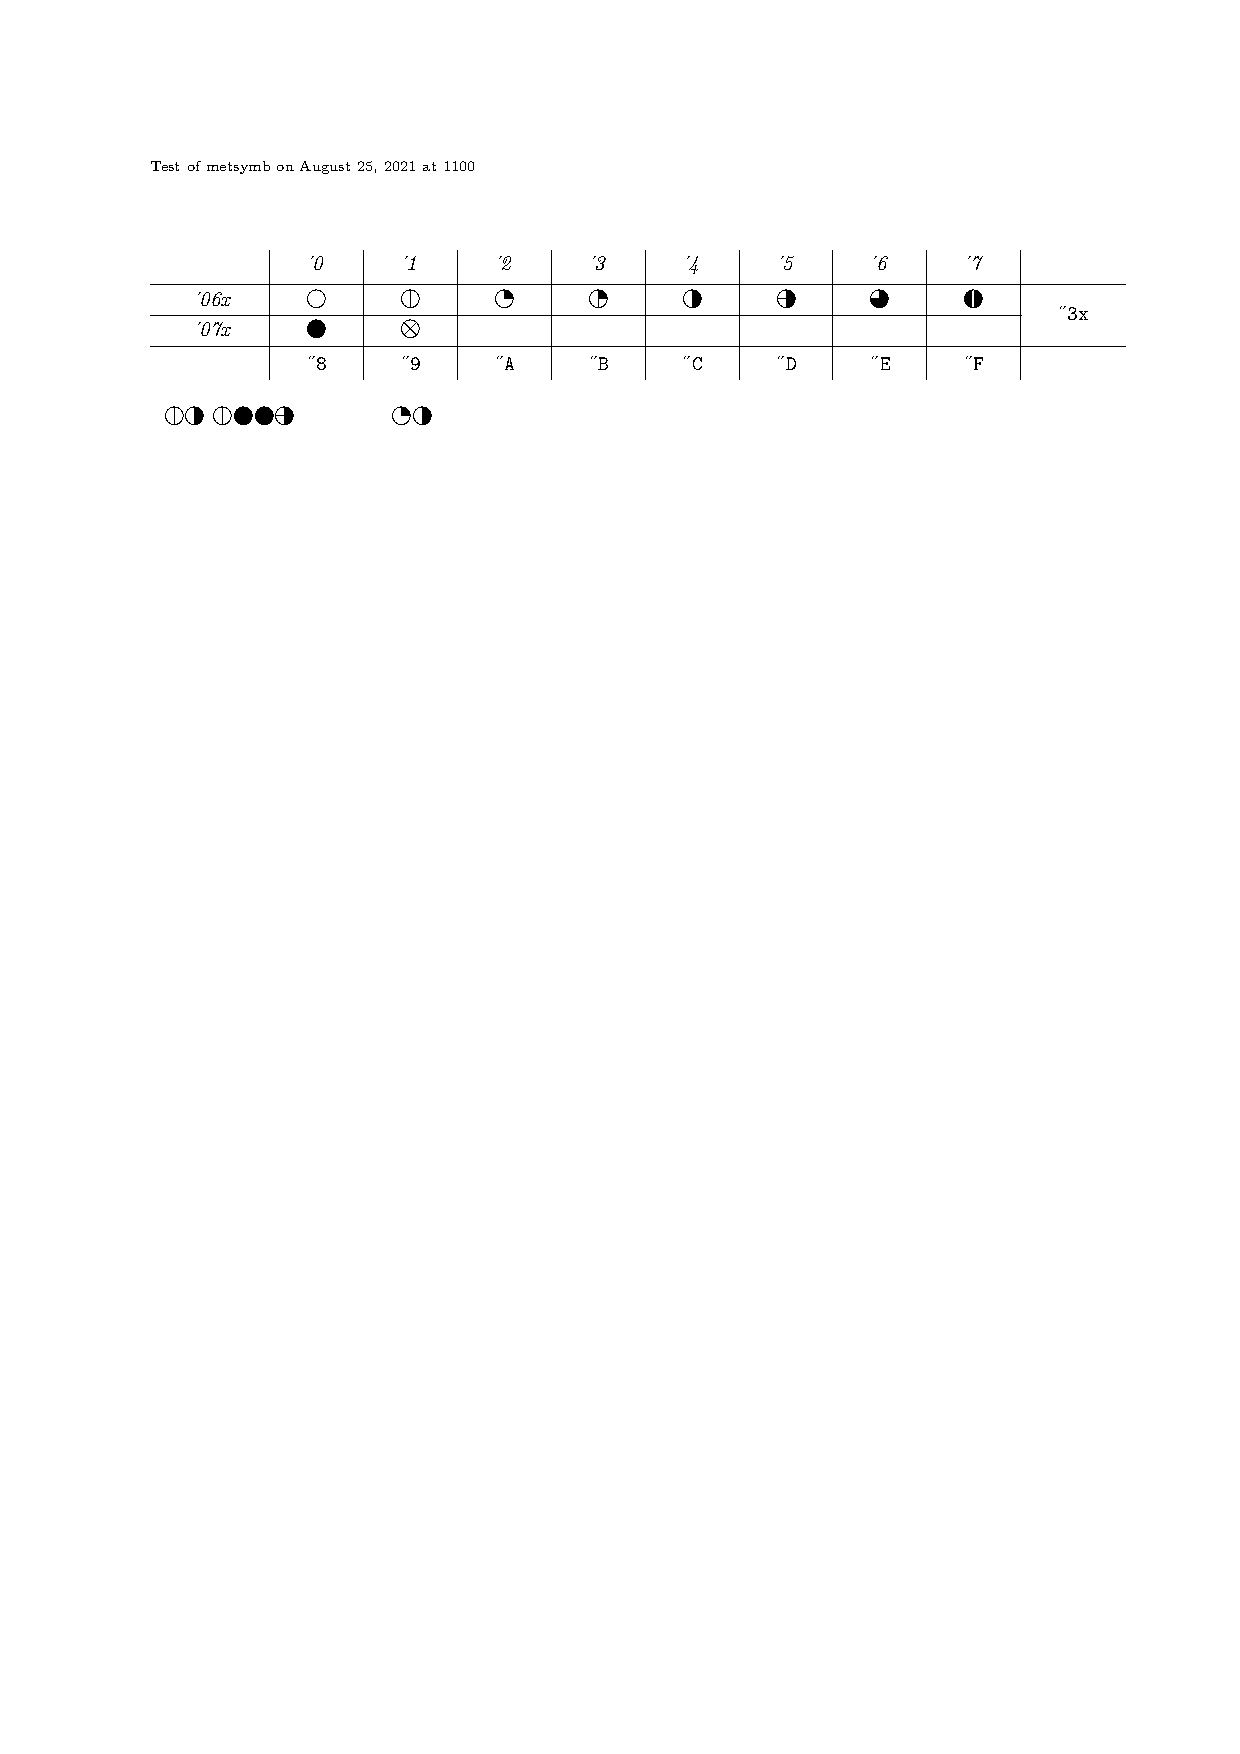
\includegraphics[scale=0.7]{testfont.pdf}}
% \caption{Complete font table for \textsf{metsymb}.}\label{fig:testfont}
% \end{figure}
%
% \StopEventually{\PrintIndex\PrintChanges}
%
% \section{Implementation}
%
% The \textsf{metsymb} package very simply defines new commands to fetch individual glyphs from the \texttt{metsymb} font. As such, its \LaTeX\ side is rather simple.
%
% \begin{macro}{\zerookta}
% The 0 okta symbol:
%    \begin{macrocode}
\newcommand{\zerookta}{{\usefont{U}{metsymb}{m}{n} 0}}%
%    \end{macrocode}
% \end{macro}
%
% \begin{macro}{\oneokta}
% The 1 okta symbol:
%    \begin{macrocode}
\newcommand{\oneokta}{{\usefont{U}{metsymb}{m}{n} 1}}%
%    \end{macrocode}
% \end{macro}
%
% \begin{macro}{\twooktas}
% The 2 oktas symbol:
%    \begin{macrocode}
\newcommand{\twooktas}{{\usefont{U}{metsymb}{m}{n} 2}}%
%    \end{macrocode}
% \end{macro}
%
% \begin{macro}{\threeoktas}
% The 3 oktas symbol:
%    \begin{macrocode}
\newcommand{\threeoktas}{{\usefont{U}{metsymb}{m}{n} 3}}%
%    \end{macrocode}
% \end{macro}
%
% \begin{macro}{\fouroktas}
% The 4 oktas symbol:
%    \begin{macrocode}
\newcommand{\fouroktas}{{\usefont{U}{metsymb}{m}{n} 4}}%
%    \end{macrocode}
% \end{macro}
%
% \begin{macro}{\fiveoktas}
% The 5 oktas symbol:
%    \begin{macrocode}
\newcommand{\fiveoktas}{{\usefont{U}{metsymb}{m}{n} 5}}%
%    \end{macrocode}
% \end{macro}
%
% \begin{macro}{\sixoktas}
% The 6 oktas symbol:
%    \begin{macrocode}
\newcommand{\sixoktas}{{\usefont{U}{metsymb}{m}{n} 6}}%
%    \end{macrocode}
% \end{macro}
%
% \begin{macro}{\sevenoktas}
% The 7 oktas symbol:
%    \begin{macrocode}
\newcommand{\sevenoktas}{{\usefont{U}{metsymb}{m}{n} 7}}%
%    \end{macrocode}
% \end{macro}
%
% \begin{macro}{\eightoktas}
% The 8 oktas symbol:
%    \begin{macrocode}
\newcommand{\eightoktas}{{\usefont{U}{metsymb}{m}{n} 8}}%
%    \end{macrocode}
% \end{macro}
%
% \begin{macro}{\nineoktas}
% The 9 oktas symbol:
%    \begin{macrocode}
\newcommand{\nineoktas}{{\usefont{U}{metsymb}{m}{n} 9}}%
%    \end{macrocode}
% \end{macro}
%
%
% \Finale
\endinput